\documentclass[aspectratio=169,10pt]{beamer}

\usepackage[T1]{fontenc}
\usepackage[utf8]{inputenc}
\usepackage[english]{babel}
\usepackage{booktabs}
\usepackage{graphicx}
\usepackage{array}

\graphicspath{{./figures/}}

\usetheme{default}
\setbeamertemplate{navigation symbols}{}
\setbeameroption{hide notes}

\definecolor{ink}{HTML}{111827}
\definecolor{muted}{HTML}{4B5563}
\definecolor{rulegray}{HTML}{D1D5DB}
\definecolor{accent}{HTML}{007A99}
\definecolor{softaccent}{HTML}{E6F6F8}

\setbeamercolor{normal text}{fg=ink,bg=white}
\setbeamercolor{frametitle}{fg=ink,bg=white}
\setbeamercolor{title}{fg=ink}
\setbeamercolor{subtitle}{fg=muted}
\setbeamercolor{author}{fg=muted}
\setbeamercolor{date}{fg=muted}
\setbeamerfont{title}{size=\Large,series=\bfseries}
\setbeamerfont{frametitle}{size=\large,series=\bfseries}
\setbeamerfont{normal text}{size=\small}
\setbeamertemplate{itemize item}{\color{accent}\raise0.2ex\hbox{\scriptsize$\blacktriangleright$}}
\setbeamertemplate{itemize subitem}{\color{accent}\raise0.2ex\hbox{\tiny$\blacktriangleright$}}
\setbeamertemplate{frametitle}{
  \vspace{0.35cm}
  \insertframetitle
  \par\vspace{0.12cm}
  {\color{rulegray}\rule{\linewidth}{0.45pt}}
}
\setbeamertemplate{footline}{
  \hfill
  {\color{muted}\scriptsize \insertframenumber/\inserttotalframenumber}
  \hspace{0.35cm}\vspace{0.18cm}
}

\newcommand{\smallcaps}[1]{{\footnotesize\bfseries\color{muted}#1}}
\newcommand{\callout}[1]{%
  \begin{beamercolorbox}[rounded=true,wd=\linewidth,sep=0.8ex]{calloutbox}
  #1
  \end{beamercolorbox}}
\setbeamercolor{calloutbox}{fg=ink,bg=softaccent}

\title{GNN-Guided Graph Partitioning for Spatial CGRA Mapping}
\subtitle{Capstone Project Final Presentation}
\author{Deniz Lopes G\"unes}
\date{June 2026}

\begin{document}

% 0:00--0:15. State the project in one sentence.
\begin{frame}[plain]
  \vspace{0.35cm}
  
\includegraphics[width=0.22\linewidth]{UPORTO_fundotransparente}

  \vfill
  {\usebeamerfont{title}\usebeamercolor[fg]{title}\inserttitle\par}
  \vspace{0.25cm}
  {\usebeamerfont{subtitle}\usebeamercolor[fg]{subtitle}\insertsubtitle\par}

  \vfill
  {\usebeamerfont{author}\insertauthor\par}
  \vspace{0.1cm}
  {\usebeamerfont{date}\insertdate\par}

  \note{This project investigates how learned graph information can guide the mapping of data-flow graphs onto coarse-grained reconfigurable arrays. The final prototype combines GNN prediction, graph partitioning, and SAT-based validation.}
\end{frame}

% 0:15--0:40. Define the compilation problem.
\begin{frame}{Problem}
  \begin{columns}[T,totalwidth=\linewidth]
    \begin{column}{0.45\linewidth}
      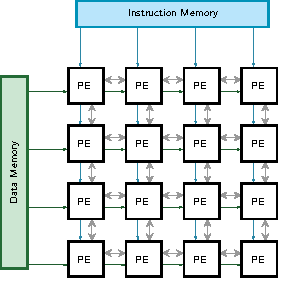
\includegraphics[width=\linewidth]{output-figure0.pdf}
    \end{column}
    \begin{column}{0.50\linewidth}
      \smallcaps{DFG-to-CGRA mapping}
      \vspace{0.25cm}
      \begin{itemize}
        \item Place graph operations on a limited grid of processing elements.
        \item Respect operation compatibility, topology, and resource constraints.
        \item Split larger graphs into feasible spatial configurations.
      \end{itemize}
      \vspace{0.25cm}
      \callout{The hard part is not only finding a placement, but choosing partitions that are likely to be mappable.}
    \end{column}
  \end{columns}

  \note{The input is a data-flow graph, and the target is a small CGRA. A mapper must assign operations to processing elements while respecting connectivity and resource limits. When the graph does not fit cleanly, partition quality becomes central.}
\end{frame}

% 0:40--1:05. Explain the idea without overloading the slide.
\begin{frame}{Direction}
  \begin{columns}[T,totalwidth=\linewidth]
    \begin{column}{0.31\linewidth}
      \smallcaps{Learn}
      \vspace{0.2cm}
      \begin{itemize}
        \item LISA showed that GNNs can predict useful graph labels.
      \end{itemize}
    \end{column}
    \begin{column}{0.31\linewidth}
      \smallcaps{Validate}
      \vspace{0.2cm}
      \begin{itemize}
        \item SAT-MapIt motivated exact constraint checking.
      \end{itemize}
    \end{column}
    \begin{column}{0.31\linewidth}
      \smallcaps{Adapt}
      \vspace{0.2cm}
      \begin{itemize}
        \item The final prototype uses one-shot spatial partitions.
      \end{itemize}
    \end{column}
  \end{columns}

  \vspace{0.65cm}
  \callout{Use the GNN to seed the partitioning decision; use SAT to verify that each resulting partition can really be mapped.}

  \note{The work started from two references: LISA for learned graph labels, and SAT-MapIt for exact mapping. Directly combining them was too broad for the capstone scope, so the project was reformulated around one-shot spatial partitioning.}
\end{frame}

% 1:05--1:35. Show the complete flow.
\begin{frame}{Implemented Flow}
  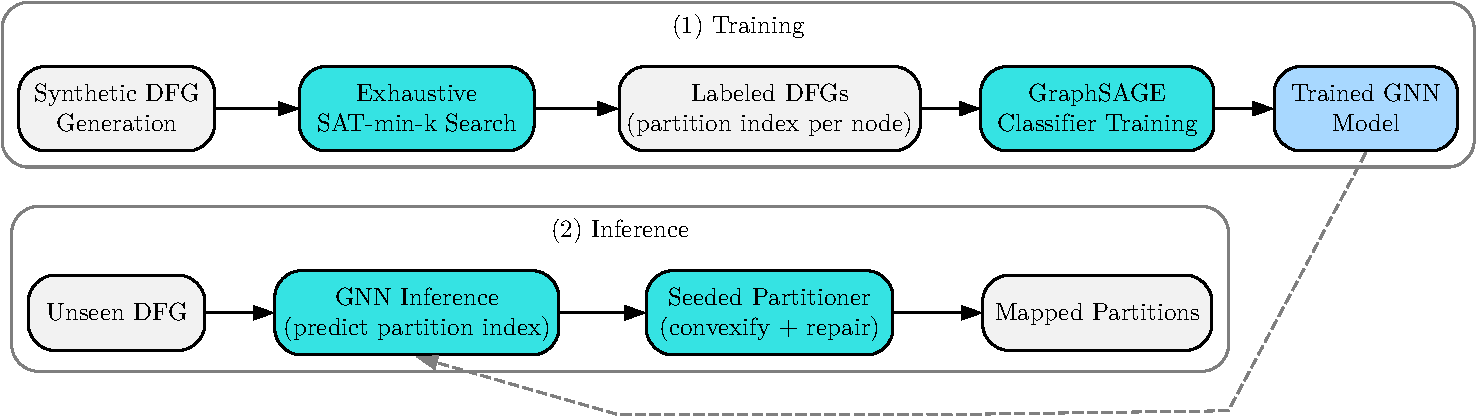
\includegraphics[width=\linewidth]{flow-crop.pdf}

  \vspace{0.25cm}
  \begin{columns}[T,totalwidth=\linewidth]
    \begin{column}{0.48\linewidth}
      \smallcaps{Training}
      \begin{itemize}
        \item Generate synthetic DFGs.
        \item Search labels with exhaustive SAT-min-k.
        \item Train a GraphSAGE classifier.
      \end{itemize}
    \end{column}
    \begin{column}{0.48\linewidth}
      \smallcaps{Inference}
      \begin{itemize}
        \item Predict partition indices.
        \item Repair infeasible predictions.
        \item SAT-map each final partition.
      \end{itemize}
    \end{column}
  \end{columns}

  \note{The offline phase generates labels by exhaustive search and trains the GNN. At inference time, the model predicts partition indices, then the topology-aware partitioner repairs the prediction before SAT validation.}
\end{frame}

% 1:35--2:00. Show data source and implementation basis.
\begin{frame}{Data and Ground Truth}
  \begin{columns}[T,totalwidth=\linewidth]
    \begin{column}{0.48\linewidth}
      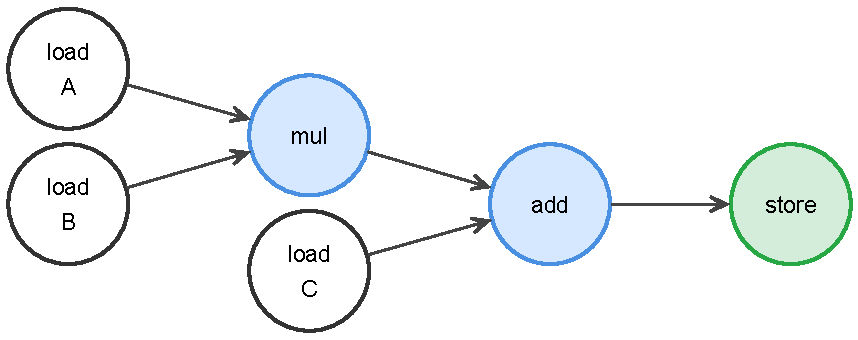
\includegraphics[width=0.98\linewidth]{matmaul_template.pdf}
      \vspace{0.15cm}
      \centering{\scriptsize Matrix multiplication template}
    \end{column}
    \begin{column}{0.48\linewidth}
      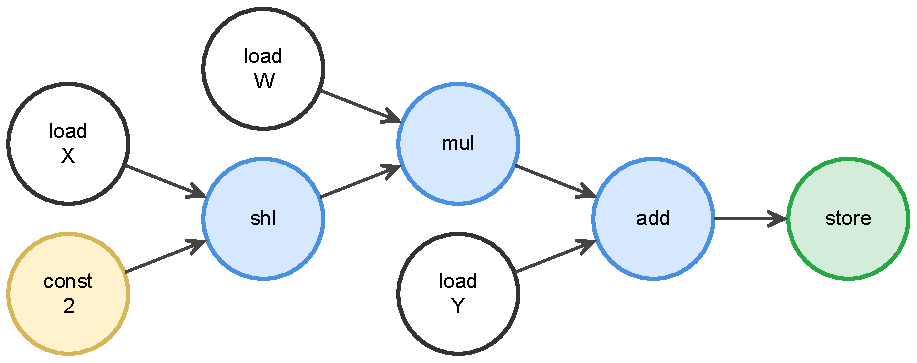
\includegraphics[width=0.98\linewidth]{conv.pdf}
      \vspace{0.15cm}
      \centering{\scriptsize Convolution template}
    \end{column}
  \end{columns}

  \vspace{0.35cm}
  \begin{itemize}
    \item 1650 synthetic DFGs generated from kernel templates.
    \item 1500 used for training and ground-truth generation; 150 held out.
    \item Labels selected by feasible partitions with minimum cuts.
  \end{itemize}

  \note{The dataset was synthetic because the project needed enough labelled graphs for training and evaluation. The labels came from the SAT-min-k process, which searches feasible partitions and keeps the best one by partition count and edge cuts.}
\end{frame}

% 2:00--2:40. Give the result in one table and one sentence.
\begin{frame}{Evaluation}
  \small
  \begin{tabular}{lccc}
    \toprule
    Strategy & Success & Mean cuts & Runtime \\
    \midrule
    SAT-min-k & 100.0\% & 1.31 & 12.1 s \\
    Greedy & 15.3\% & 1.52\textsuperscript{\dag} & 0.08 s \\
    Topological repair & 92.7\% & 3.22 & 0.51 s \\
    GNN-raw & 70.7\% & 1.74 & 0.07 s \\
    \textbf{GNN-guided} & \textbf{98.0\%} & \textbf{2.15} & \textbf{0.25 s} \\
    \bottomrule
  \end{tabular}

  \vspace{0.25cm}
  {\scriptsize \textsuperscript{\dag}Greedy cuts are reported only on its successful cases. Runtime is partitioning plus SAT mapping.}

  \vspace{0.45cm}
  \callout{GNN-guided repair reached 147/150 mapped graphs and reduced cuts relative to unguided topological repair, while staying about 50$\times$ faster than exhaustive search.}

  \note{The exhaustive method is the quality reference but is much slower. Raw GNN predictions are fast but unreliable. The best practical strategy was GNN-guided repair, which mapped 98 percent of the evaluation set and reduced cuts compared with topology-only repair.}
\end{frame}

% 2:40--3:00. Close with contribution and limits.
\begin{frame}{Takeaway}
  \begin{columns}[T,totalwidth=\linewidth]
    \begin{column}{0.55\linewidth}
      \smallcaps{Main contribution}
      \vspace{0.25cm}
      \begin{itemize}
        \item A working DFG-to-CGRA mapping pipeline.
        \item SAT-generated supervision for a learned partitioner.
        \item Feasibility repair tied to CGRA topology.
      \end{itemize}
    \end{column}
    \begin{column}{0.38\linewidth}
      \smallcaps{Current scope}
      \vspace{0.25cm}
      \begin{itemize}
        \item Homogeneous $4\times4$ CGRA.
        \item Synthetic DFGs.
        \item One-shot spatial mapping.
      \end{itemize}
    \end{column}
  \end{columns}

  \vspace{0.65cm}
  \callout{The result is not a replacement for exact mapping; it is a faster way to guide partitioning before exact validation.}

  \note{The project produced the generator, exact labelling flow, GNN predictor, topology-aware repair step, SAT mapper, and benchmark. The main limitation is scope: future work should test compiler-derived DFGs, larger or heterogeneous CGRAs, and temporal scheduling.}
\end{frame}

\end{document}
